\documentclass[10pt,a4paper]{article}	
\usepackage{amsmath}
\usepackage{amsfonts}
\usepackage{amssymb}
\usepackage{cite}												% 支持引用多篇文献
\usepackage{CJK}													% 支持中文
\usepackage{indentfirst}                 						% 首行缩进宏包
\usepackage{graphicx}											% 支持图片的插入
\usepackage{subfigure}											% 支持插入子图
\usepackage[colorlinks,citecolor = blue, linkcolor=blue,hyperindex,CJKbookmarks]{hyperref}	% 链接功能
\usepackage{fancyhdr}											% 添加页眉
\usepackage{array}												% 使用表格
\usepackage{multirow}

\newcommand{\PreserveBackslash}[1]{\let\temp=\\#1\let\\=\temp}	% 表格固定
\newcolumntype{C}[1]{>{\PreserveBackslash\centering}p{#1}}		% 宽度并且
%\newcolumntype{R}[1]{>{\PreserveBackslash\raggedleft}p{#1}} 		% 使用居中
%\newcolumntype{L}[1]{>{\PreserveBackslash\raggedright}p{#1}}		% 排列方式
\graphicspath{{figs/}}                              				% 图片文件夹路径
\setlength{\parindent}{2em}										% 缩进距离为2个字符位置
\newcommand{\song}{\CJKfamily{song}}     						% 宋体
\newcommand{\hei}{\CJKfamily{hei}}       						% 黑体
\newcommand{\fs}{\CJKfamily{fang}}         						% 仿宋
\newcommand{\kai}{\CJKfamily{kai}}       						% 楷体
\newcommand{\li}{\CJKfamily{li}}         						% 隶书
\newcommand{\you}{\CJKfamily{you}}       						% 幼圆


\begin{document}

\begin{CJK*}{UTF8}{gkai}
%============================++题目和作者++================================
\pagestyle{fancy} 
\lhead{}
\chead{\small{同济大学高级管理学课程报告}}
\rhead{}
\title{组织政治知觉对IT行业知识型员工影响的研究综述}					% 题目
\author{郝俊禹\thanks{学院:电信院;\;专业:计算机技术;\;学号:1333885;\;Email:haojunyu2012@gmail.com}}									% 作者
%============================++++++++++++=================================
\date{}                                             				% 显示作者,不显示日期
\maketitle                                          				% 生成标题
\tableofcontents 												% 生成目录
\clearpage


\section{引言}
在当今的经济发展与企业竞争中,人力资源已经成为组织中最重要的资源。企业的
知识型员工是企业人力资源的核心,是企业核心竞争能力的体现,是衡量一个企业的发
展能力的重要指标。知识型员工的巨大价值还在于其利用自身独有的知识,处理复杂性
和不确定性问题的能力。知识型员工为组织获得竞争优势及稳定增长方面起到不可替代
的重要作用,如果知识型员工没有被有效地管理,他们就不能发挥出独特的作用。


对于IT行业这种新型产业来说,知识型员工的作用更加明显。因此,能否激发知识型员工
的工作热情,提高知识员工的创造力与潜能,培养他们的责任感,改善和促进知识、
技术的生产、传播、应用和增值,直接决定了IT企业能否在日新月异的知识更新和激烈的
行业内竞争中处于不败之地。但是,由于企业资源永远都是稀缺的,不可能满足每一个
员工都获得其想拥有的利益。另外,由于现代社会经济环境的剧烈变化和飞速发展,
加剧了社会和企业环境的不确定性等因素,为组织政治的产生和蔓延创造了充分的空间。


在包括企业在内的任何组织中,组织政治及其影响几乎无处不在,甚至在有些组织中代替了
组织的正式规则,成为组织中心照不宣、人人遵守、无人能违背的分配资源的规则。
国外的现有研究成果表明,组织政治对员工的工作满意度、离职意图、心理应激和工作绩效等
有重要影响。因此,对企业内的组织政治进行研究,降低其负面影响,提高员工的工作满意度,
降低离职率,充分凋动其工作积极性都具有重大意义。员工对组织政治的感知和反应,也就是
组织政治知觉,也成为国内外众多学者研究的对象。尤其是企业知识型员工的组织政治知觉,
对企业的长久生存、目标的实现和有效地管理人力资源等众多方面都至关重要。


\section{相关概念及历史}
\subsection{IT行业的定义及特点}
IT(Information Technology)是信息技术的简称,是主要用于管理和处理信息所采用的各种技术总称。它主要是应用计算机科学和通信技术来设计、开发、安装和实施信息系统及应用软件。它也常被称为信息和通信技术(Information and Communications Technology, ICT)\cite{1}。IT在二十世纪的现在已经成为各行各业的公用技术,因为任何管理活动都离不开对信息的依赖。IT的普遍应用,是进入信息社会的标志。

IT行业主要包括:传统的硬件制造业、软件企业、网络服务业和系统集成企业等。与其他产业相比,IT行业有以下突出特点:
\begin{enumerate}
\item 高智力密集型、高技术性\\
IT企业是最典型的技术密集型、知识密集型的产业,人才是IT企业最宝贵的财富,
具有明显的技术性、稀缺性、流动性和年轻化的特点。
\item 高投入、高风险、高收益\\
IT企业在产品研发、生产和市场推广过程中,都要进行巨额的资金、设备和人力投
入,由于技术的高度复杂性和市场的高度不确定性,项目风险控制难度加大,项目的成
功率较低。但是一旦某个新项目或新产品获得成功,将会带来相对高额的回报。
\item 高时效性\\
IT企业组织管理模式日新月异,产品生命周期越来越短,市场变化越来越快。能否
适应技术、市场和管理的快速变化,不断地进行创新,比竞争对手更快地推出产品或占
领市场,将直接决定IT企业的成败。
\item 高竞争性\\
目前,IT行业内部竞争空前激烈,随着IT技术的发展,竞争对手更加具有一定程
度的不可预测性。
\end{enumerate}


\subsection{知识型员工的概念及特点}
知识型员工是美国学者彼得·德鲁克发明的,指的是那些掌握和运用符号和概念,利用知识或信息工作的人。其实当时他指的是某个经理或执行经理。在今天,知识型员工实际上已经被扩大到大多数白领。企业之间的竞争,知识的创造、利用与增值,资源的合理配置,最终都要靠知识的载体——知识型员工来实现。知识型员工的特点,用一句话来概括就是:作为追求自主性、个体化、多样化和创新精神的员工群体,激励他们的动力更多的来自工作的内在报酬本身。\cite{2}


综合国内外学者如德鲁克(Druke,1999)、彭剑锋(2001)、张望军(2001)等人的观点,结合IT行业的行业特点,IT行业知识型员工的特点主要有以下几点\cite{3}:
\begin{enumerate}
\item 员工年轻化\\
IT企业从业人员是伴随改革开放和高新技术发展而形成的一个新型群体。lT企业
是年轻人聚集的地方,往往充满着活力和热情。IT企业的研发人员以20至30岁年龄段
为主。许多IT企业的中高层管理人员年龄也明显比其他行业人员低。
\item 有较强的自主意识\\
一般人都有独立自主的要求,能力越强,独立自主从事某项活动的意识就越强。由
于IT行业知识型员工具有特殊的技能,他们往往倾向于一个自主的工作空间,去做他
们自己喜欢做的事。在组织中,他们一般不愿受制于他人,甚至是领导。他们强调工作
中的自我引导,对各种可能性做最大的尝试,不愿俯首听命,任人驾驭。
\item 有独立的价值观\\
与一般员工相比,IT行业知识型员工更有一种表现自己的强烈欲望。他们为企业工
作,并不仅仅为了挣钱,而是更关心能否发挥自己专长、实现个人理想。他们更在意自
身价值的实现,并期望得到社会的认可。因此,他们热衷于具有挑战性的工作,把攻克
难关看作一种乐趣,一种体现自我价值的方式。
\item 较强的创新精神和知识创新能力\\
知识创新能力是IT行业知识型员工最主要的特点。IT行业知识型员工之所以重要,
并不仅仅因为他们掌握了某些核心知识,还因为他们具有不断创新知识的能力。IT行业
知识型员工面对的是多变的、不确定的环境,因此他们的工作不具有常规性,也没有太
多可以参照的模本,是在易变和不完全确定的系统中充分发挥个人的才干和灵感。与体
力劳动者或一般事务人员相比,IT行业知识型员工更可能遇到不可预见的问题,如何解
决新问题或突发性问题就成为IT行业知识型员工存在的价值所在,这也是IT行业知识
型员工不可替代的原因。
\item 有较强的流动意愿\\
IT行业知识型员工不属于某一个特定组织,而属于那些能够最大满足他们需要的组
织。对IT行业知识型员工而言,寻求一个更适合自己发展和学习提高的环境,是保证
其知识资本不贬值的必然选择。他们最关心的问题就是不断地提高自己的知识水平,以
适应激烈竞争的需要。因此,组织能否提供知识更新和培训机会就成为IT行业知识型
员工选择去留的重要原因,当组织不能满足他们自我实现的需要时,他们会毫不犹豫地
跳槽而去\cite{4}。
\end{enumerate}

\subsection{组织政治的概念及模型}
关于组织政治行为的概念,不同的学者从不同的角度给出了不同的定义。
Mintzberg(1985)认为组织是政治支配的竞技场;而Drory(1988)认为政治行为并非
组织成员本身职责所要求的活动,却可以影响组织内部利益的分配。由于其存在
的普遍性,组织政治已然是现代组织生活的一部分(Ferris\&{}
Kacmar,1992)。比如说,在组织运作过程中,与员工切身利益相关的许多人力资
源的决策,最常见的像加薪和晋升等问题,都会受到政治行为的潜在影响。


组织政治知觉的相关研究相对起步较晚,目前被最广泛使用的组织政治知觉
模型是Ferris等人(1989)研究组织政治知觉时所建立的,如图\ref{fig:1};此后大多学
者的研究都是在该模型的基础上展开\cite{6}。
\begin{figure}[!htbp]
	\centering
	\caption{组织政治知觉模型}  
		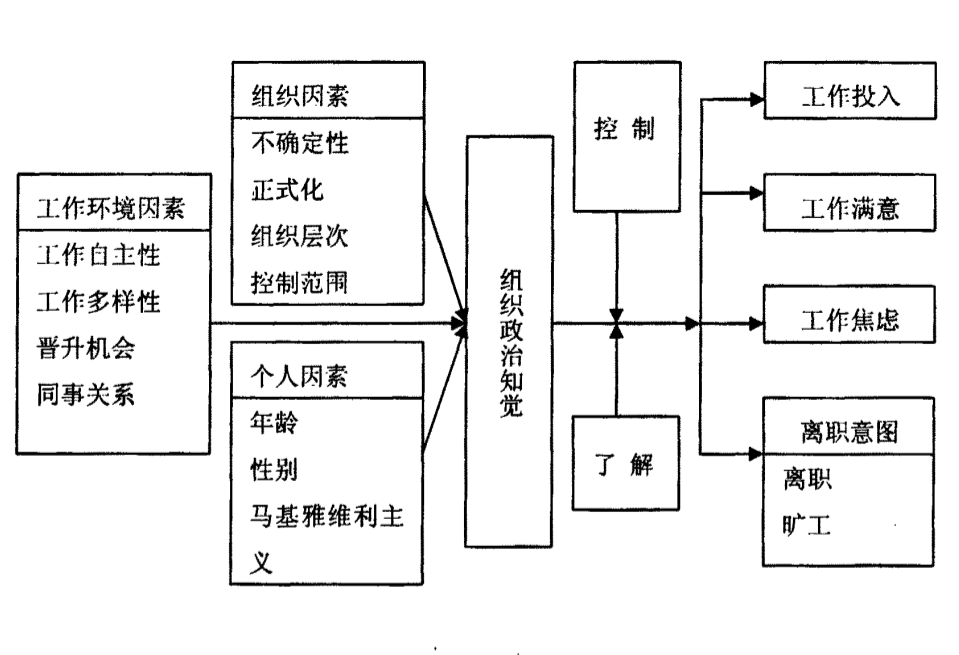
\includegraphics[scale=0.45]{figs/1.png}
    	\label{fig:1}
\end{figure}



\section{组织政治知觉的相关变量}
在最近的二十年中,学者们的相关研究极大的丰富和发展了Ferris的组织政
治知觉模型,验证并新提出了许多组织政治知觉的相关变量。
\subsection{前因变量}
Kacmar和Baron(1999)认为组织政治行为是直接由个人发动的,所以很多
组织政治知觉前因变量的研究都是从个体的角度出发,当然从组织和工作环境因
素出发的研究也不少见。组织政治知觉与其前因变量的关系如下表\ref{tab:1}:
\begin{table}[!htp]
\label{tab:1}
\center
\begin{tabular}{C{2.5cm}|C{4.5cm}|C{3cm}}
\hline
前因变量 	& 	学者 	& 	结果		\\ 
\hline
年龄 & Kacmar \&{} Ferris,1992 & 正相关\\
\hline
\multirow{2}{*}{受教育程度}  & Parker 等,1995  & 正相关\\
\cline{2-3}
       & Vigoda \&{}Cohen,2002  & 负相关\\
\hline
\multirow{3}{*}{性别}  & Drory,1993  & 不显著\\
\cline{2-3}
       & Ferris,Frink \&{}Bhawuk,1996  & 负相关\\
\cline{2-3}
       & Vigoda \&{}Cohen,2002  & 显著(女性高)\\
\hline
\multirow{2}{*}{薪酬}  & Kacmar \&{} Ferris,1992 & 负相关\\
\cline{2-3}
        & Ferris,Frink \&{}Bhawuk,1996  & 正相关\\
\hline
马基雅维利主义 & Valle \&{}Perrewe,2000 &  正相关\\
\hline
\multirow{2}{*}{工作自主性}  & Kacmar \&{} Ferris,1992 & \multirow{2}{*}{负相关}\\
\cline{2-2}
        & Valle \&{}Perrewe,2000 &  \\
\hline
\multirow{2}{*}{工作多样性}  & Kacmar \&{} Ferris,1992 & \multirow{2}{*}{负相关}\\
\cline{2-2}
        & Valle \&{}Perrewe,2000 &  \\
\hline
反馈 & Kacmar,Bozeman \&{}Carison,1999 &  负相关\\
\hline
\multirow{2}{*}{晋升机会}  & Kacmar,Bozeman \&{}Carison,1999 & \multirow{2}{*}{负相关}\\
\cline{2-2}
        & Valle \&{}Perrewe,2000 &  \\
\hline
\multirow{2}{*}{与上司的关系}  & Kacmar \&{} Ferris,1992 & \multirow{2}{*}{负相关}\\
\cline{2-2}
        & Valle \&{}Perrewe,2000 &  \\
\hline
\multirow{2}{*}{集权化}  & Kacmar,Bozeman \&{}Carison,1999 & 负相关\\
\cline{2-3}
        & Valle \&{}Perrewe,2000 &  正相关\\
\hline
正式化 & Kacmar \&{} Ferris,1992 & 负相关\\
\hline
\multirow{2}{*}{等级地位}  & Drory,1993 & 正相关\\
\cline{2-3}
        & Valle \&{}Perrewe,2000 &  负相关\\
\hline
\end{tabular}
\end{table}

\subsection{结果变量}
十几年来学者对组织政治知觉的结果变量的研究成果也十分丰硕。其结果如下表\ref{tab:2}:
\begin{table}[!htp]
\label{tab:2}
\center
\begin{tabular}{C{2.5cm}|C{4.5cm}|C{3cm}}
\hline
结果变量 	& 	学者 	& 	结果		\\ 
\hline
\multirow{2}{*}{工作投入}  & Kacmar \&{} Ferris,1992 & 负相关\\
\cline{2-3}
        & Cropanzano等,1997 &  正相关\\
\hline
\multirow{2}{*}{工作满意}  & Parker等,1995 & \multirow{2}{*}{负相关}\\
\cline{2-2}
        & Poon,2003 &  \\
\hline
\multirow{3}{*}{工作焦虑}  & Kacmar,Bozeman \&{}Carison,1999  & \multirow{3}{*}{正相关}\\
\cline{2-3}
       & Valle \&{}Perrewe,2000  & \\
\cline{2-3}
       & Poon,2003  & \\
\hline
\multirow{3}{*}{离职意图}  & Kacmar,Bozeman \&{}Carison,1999  & \multirow{3}{*}{正相关}\\
\cline{2-3}
       & Valle \&{}Perrewe,2000  & \\
\cline{2-3}
       & Poon,2003  & \\
\hline
\end{tabular}
\end{table}

\subsection{缓冲变量}
鉴于组织政治知觉与各结果变量的关系会受到各缓冲变量的影响,近十几年
来许多学者加强了对缓冲变量的研究。如下表\ref{tab:3}:
\begin{table}[!htp]
\label{tab:3}
\center
\begin{tabular}{C{2.5cm}|C{4.5cm}|C{3cm}}
\hline
缓冲变量 	& 	学者 	& 	结果		\\ 
\hline
了解  &  Kacmar,1999  & 成立\\
\hline
控制  &  Poon,2004    & 成立\\
\hline
\end{tabular}
\end{table}

\section{研究意义及挑战}
\subsection{研究意义}
文献\cite{7}采用实证研究的方法,通过问卷调查,对IT企业知识型员工的
组织政治知觉和大五人格特质进行了测量,通过SPSS统计学工具,验证了事先提出的
假设的合理性。最后,根据研究结果认为,IT企业应及时对员工进行心理测试,
把握员工心理动向和人格倾向,做好员工心理辅导;另外,建立一个具有凝聚力的企业
文化,并做好相关的培训,这样就能够有效地减小知识型员工组织政治知觉对其工作绩
效产生的不良影响。


文献\cite{8}通过访谈和预调研验证构思及修改了问卷;最后是问卷研究,在对杭州、
上海等城市的IT企业员工进行问卷调查的基础上,利用SPSSl3.0的分析结果迸一步
验证研究的构思模型。得出IT企业员工的压力感知处于中等水平,组织政治知觉可以有效地预测员工的压力水平等结论。


文献\cite{9}通过对组织政治知觉和员工行为的各自的含义、结构进行深入研究总结。
并且总结了国外组织政治知觉和员工行为的相关研究结果,最后 
就如何减少组织政治知觉对员工行为的影响提出了几点粗浅的建议 。
 


\subsection{研究挑战}
目前,对于组织政治知觉对IT行业知识型员工影响的研究依旧还有很多的角度可以出发,以上的文献中
有从大五人格和组织政治知觉的关系进行研究,也有从组织公平和组织政治知觉的关系进行研究等。针对
这个有着高智力密集型、高技术性、高投入、高风险、高收益、高时效性、高竞争性等特点的IT行业,面对这这样一群年轻化、有较强自主意识、有独立价值观、有较强创新精神和知识创新能力、有较强流动意愿的知识型员工,组织政治知觉所起的影响是多方面的,而且是有侧重点的。所以从多个不同的方向发掘其的作用是有意义的,能够促进IT企业对其核心的知识型员工的有效管理;能够让员工对自身组织政治知觉程度尽早有所了解,并消除对他们工作绩效的不良影响具有实际意义;能够帮助IT类企业了解
其知识型员工的现状,为IT类企业人力资源管理提供参考;能够提高知识型员工的绩效,激发他们的工作热情和创新意识,使他们发挥出最大的能量为企业发展做出贡献。
		
		
\bibliographystyle{unsrt}										% 按引用的先后顺序排列,比较次序为作者,年度和标题
\bibliography{ref/mybib}												% 引用文件数据库在bib.bib文件中

\clearpage     
\end{CJK*}
\end{document}
